\chapter{Database MySQL}

\section{Pengenalan Database MySQL pada Java}

\subsection{Pendahuluan}

MySQL adalah salah satu sistem manajemen basis data relasional (RDBMS) yang paling populer di dunia. MySQL digunakan secara luas karena kecepatan, skalabilitas, dan kemudahan penggunaannya. Dalam pengembangan aplikasi Java, MySQL sering digunakan sebagai database untuk menyimpan dan mengelola data. Untuk menghubungkan aplikasi Java dengan MySQL, kita menggunakan Java Database Connectivity (JDBC).

\subsection{Langkah-langkah Menggunakan MySQL di Java}

Berikut adalah langkah-langkah untuk menghubungkan aplikasi Java dengan database MySQL:

\subsubsection{1. Instalasi MySQL}

Sebelum memulai, pastikan Anda telah menginstal MySQL di sistem Anda. Anda dapat mengunduh dan menginstalnya dari situs web resmi MySQL.\\

Silahkan tonton video berikut untuk panduan lebih lanjut\\ \url{https://www.youtube.com/watch?v=Ev_h-6OkvA4&list=PLl9D0-J08TNXNjQPwWMVOUrqA-oiDrGyk&index=13}

\subsubsection{2. Menyiapkan Database MySQL}

Setelah MySQL terinstal, Anda dapat membuat database yang akan digunakan dalam aplikasi Java Anda. Misalnya, kita akan membuat database \texttt{studentdb} dan tabel \texttt{students} untuk menyimpan data mahasiswa. 

Untuk bagian ini, kamu dapat membuat database dengan alternatif seperti PHPMyAdmin, DBeaver, atau MySQL Workbench(Hanya untul SQL versi 8.5 kebawah). Bahkan kamu juga bisa membuat tabel dengan command prompt saja (lihat pada link youtube untuk tata cara dengan MySQL Workbench)

\subsubsection{2.1 Persiapan Database dengan MySQL dan DBeaver}

Sebelum memasuki persiapan ini, pastikan telah menonton video untuk mengetahui cara mengaktifkan koneksi dengan CLI (Command Line).

\begin{itemize}
	\item Download Dbeaver melalui link berikut \\ \url{https://dbeaver.io/download/}
	
	\item Setelah instalasi telah dilakukan, buka Dbeaver
	
	\item Pada bagian kiri atas, pilih New Database Connection
	
	\item Pilih MySQL , kemudian klik Next\\
	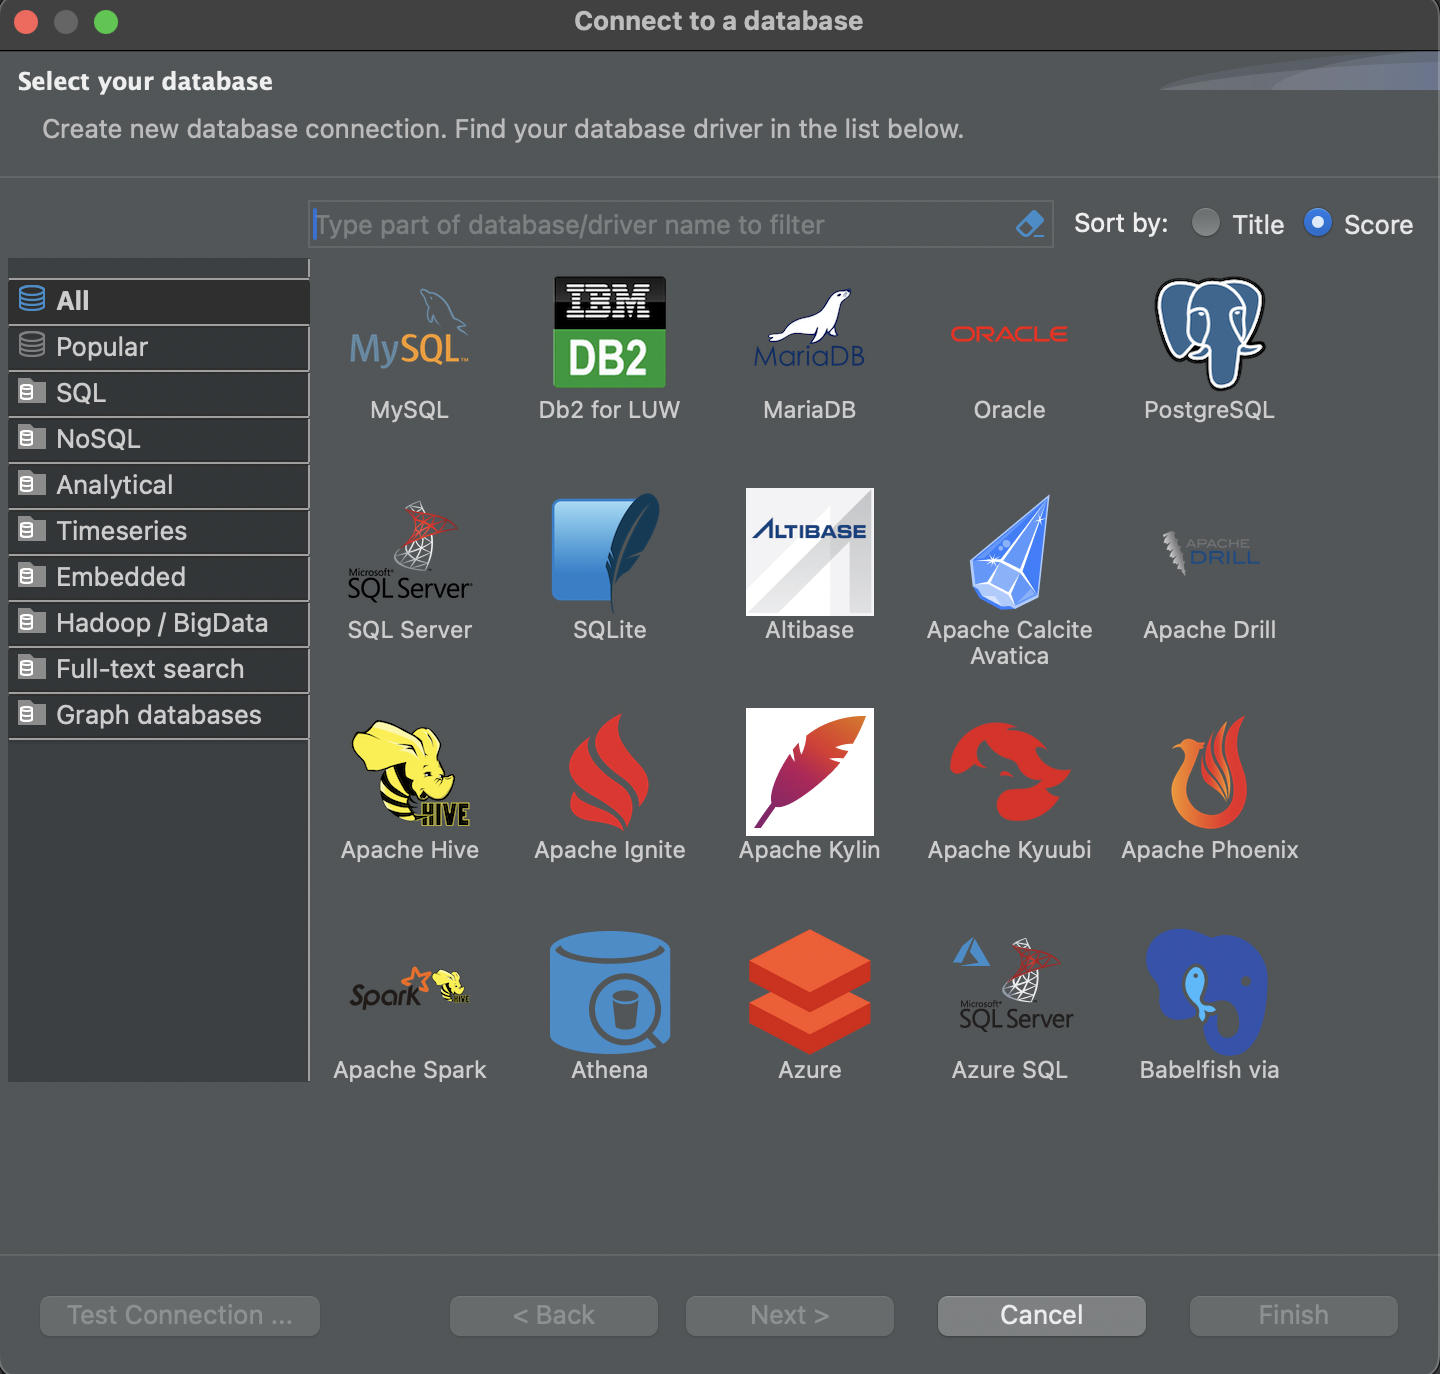
\includegraphics[width=0.33\textwidth]{assets/pertemuan12/dbeaver-select-connection.png}
	
	\item Pada halaman Connection Settings, tidak perlu mengubah konten yang ada, langsung klik Finish\\
	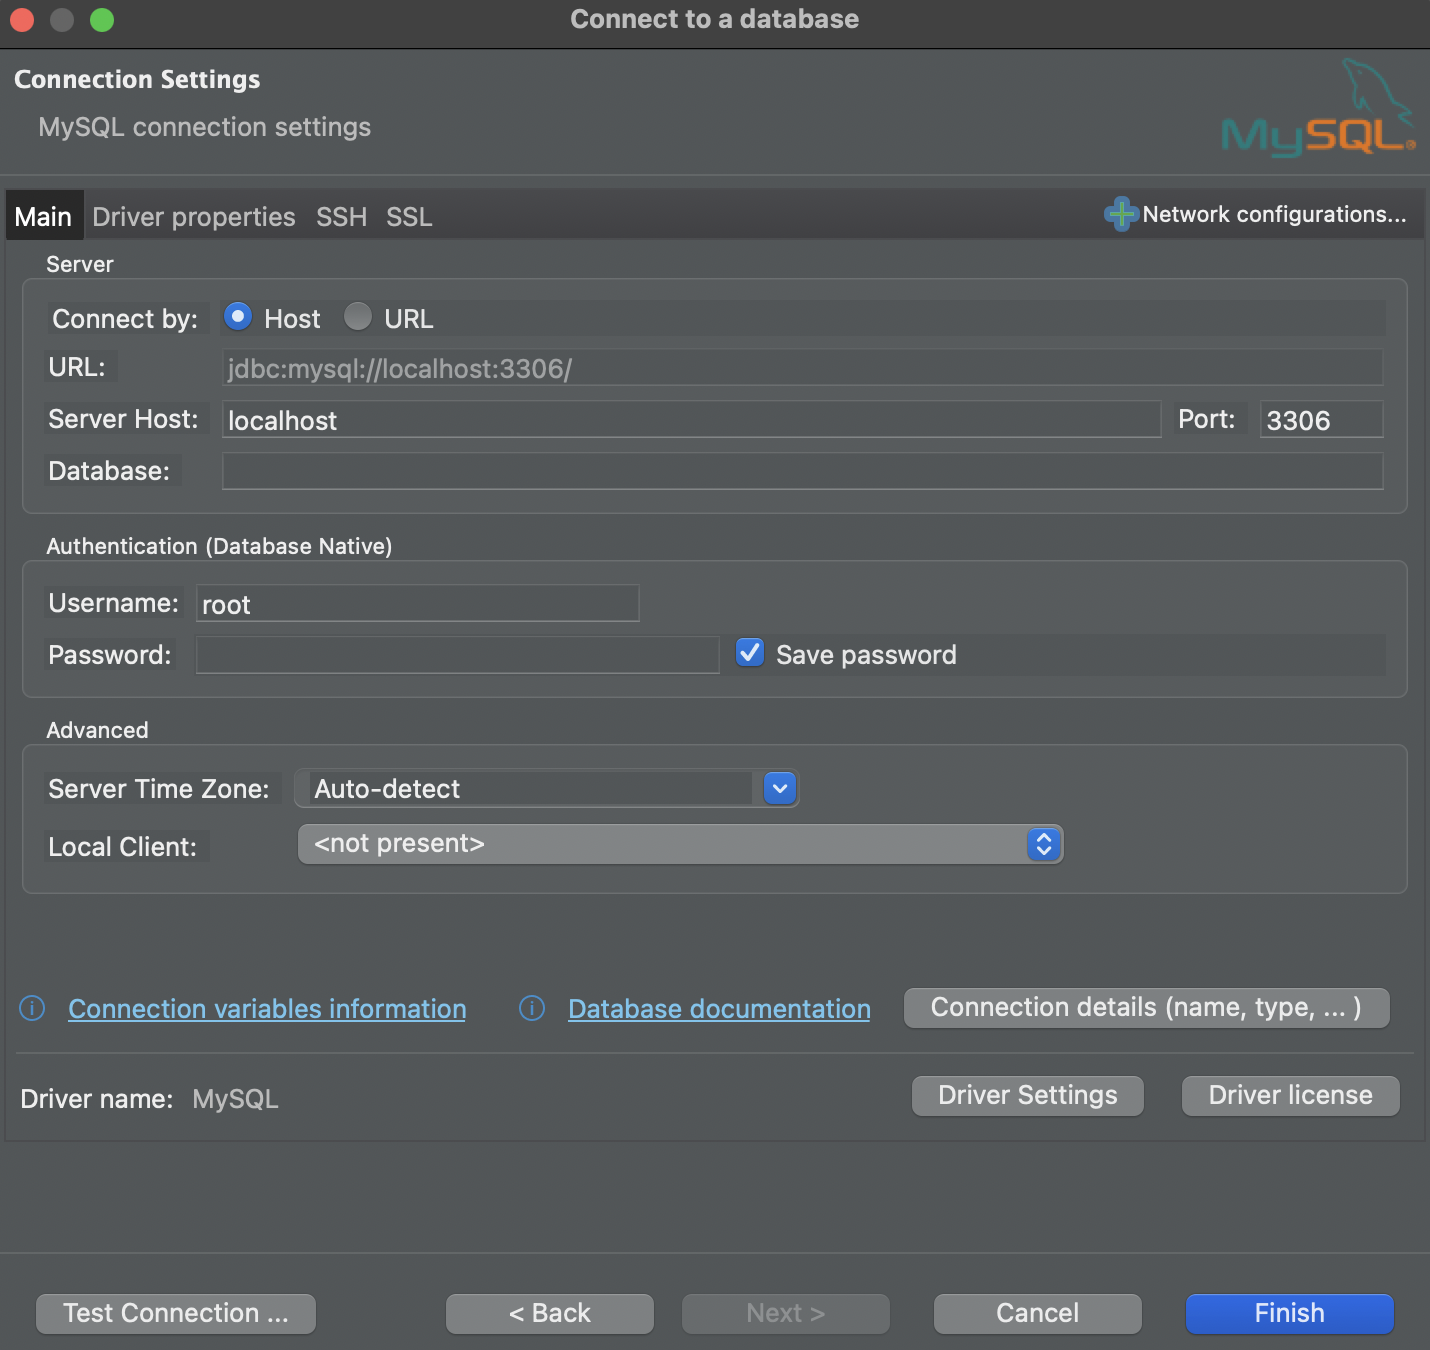
\includegraphics[width=0.33\textwidth]{assets/pertemuan12/dbeaver-connection-settings.png}
	
	\item Setelah telah terkoneksi, expand bagian koneksi yang telah dibuat 
	
	\item Expand menu Databases
	
	\item Klik kanan pada menu Databases, kemudian pilih Create New Databases
	
	\item Masukkan nama studentdb pada nama database, kemudian klik OK
	
	\item Pada nama database studentdb, klik kanan, pilih SQL Editor dan pilih create New Script
	
	\item Masukkan script berikut, kemudian run
	\begin{lstlisting}[style=JavaStyle]
		USE studentdb;
		
		CREATE TABLE students (
			id INT AUTO_INCREMENT PRIMARY KEY,
			name VARCHAR(50),
			age INT,
			major VARCHAR(50)
		);
	\end{lstlisting}
	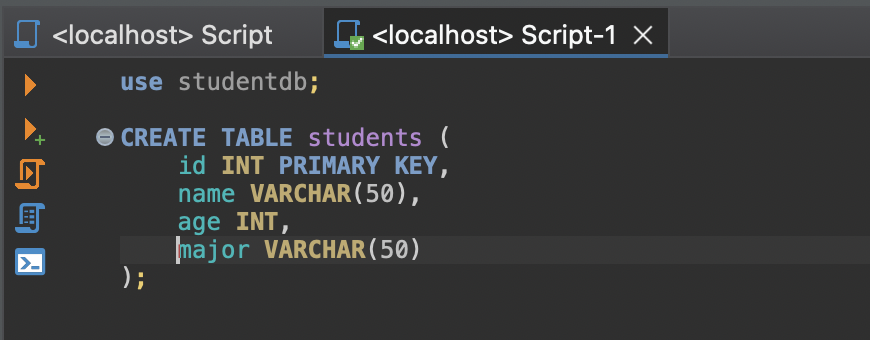
\includegraphics[width=0.33\textwidth]{assets/pertemuan12/dbeaver-script-create-table.png}
	
	\item Database dan table sudah berhasil dibuat!\\
	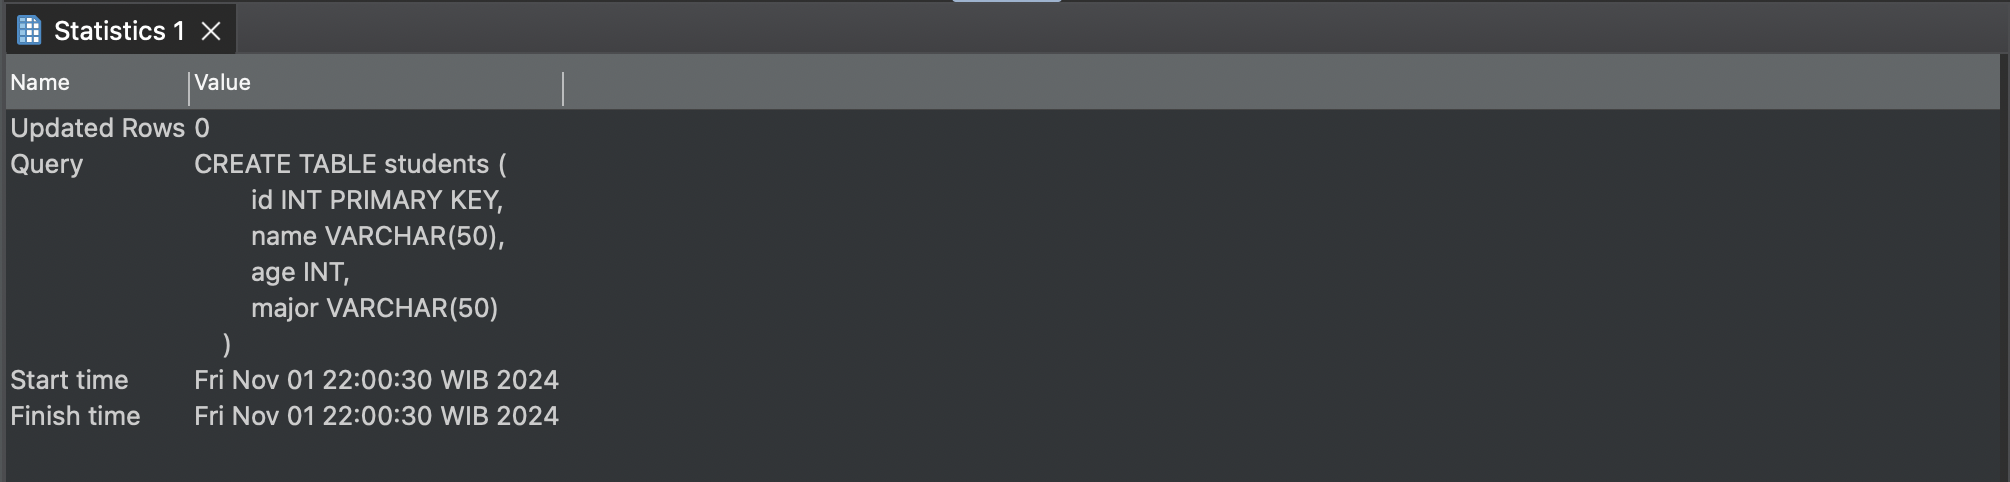
\includegraphics[width=0.8\textwidth]{assets/pertemuan12/dbeaver-table-success-script.png}
	
\end{itemize}

\subsubsection{3. Menambahkan MySQL Connector ke Proyek Java}

Agar aplikasi Java dapat berkomunikasi dengan MySQL, Anda perlu menambahkan \texttt{MySQL Connector/J} ke dalam proyek Anda. \texttt{MySQL Connector/J} adalah driver JDBC yang menyediakan koneksi antara Java dan MySQL.

\begin{enumerate}
	\item Unduh \texttt{MySQL Connector/J} dari situs web MySQL.
	\item Tambahkan file \texttt{.jar} ke dalam build path proyek Java Anda.
	\begin{itemize}
		\item Jika menggunakan Eclipse, klik kanan pada proyek Anda > \texttt{Properties} > \texttt{Java Build Path} > \texttt{Libraries} > \texttt{Add External JARs...} > pilih \texttt{mysql-connector-java-x.x.xx-bin.jar}.
	\end{itemize}
\end{enumerate}

\subsubsection{4. Menghubungkan Java dengan MySQL Menggunakan JDBC}

Berikut adalah contoh sederhana untuk menghubungkan Java dengan MySQL menggunakan JDBC:

\begin{lstlisting}[style=JavaStyle]
	import java.sql.Connection;
	import java.sql.DriverManager;
	import java.sql.ResultSet;
	import java.sql.Statement;
	
	public class MySQLConnectionExample {
		public static void main(String[] args) {
			String url = "jdbc:mysql://localhost:3306/studentdb";
			String username = "root";
			String password = "password";
			
			try {
				// Membuat koneksi ke database
				Connection conn = DriverManager.getConnection(url, username, password);
				System.out.println("Koneksi berhasil!");
				
				// Membuat statement
				Statement stmt = conn.createStatement();
				
				// Mengeksekusi query
				String sql = "SELECT * FROM students";
				ResultSet rs = stmt.executeQuery(sql);
				
				// Menampilkan hasil query
				while (rs.next()) {
					System.out.println("ID: " + rs.getInt("id"));
					System.out.println("Name: " + rs.getString("name"));
					System.out.println("Age: " + rs.getInt("age"));
					System.out.println("Major: " + rs.getString("major"));
					System.out.println("-------------");
				}
				
				// Menutup koneksi
				conn.close();
			} catch (Exception e) {
				e.printStackTrace();
			}
		}
	}
\end{lstlisting}

\subsection{Penjelasan Kode}

\begin{itemize}
	\item \texttt{DriverManager.getConnection(url, username, password);} - Digunakan untuk membuat koneksi ke database MySQL.
	\item \texttt{Statement stmt = conn.createStatement();} - Membuat statement untuk menjalankan query SQL.
	\item \texttt{ResultSet rs = stmt.executeQuery(sql);} - Mengeksekusi query SQL dan menyimpan hasilnya dalam objek \texttt{ResultSet}.
	\item \texttt{rs.getInt(), rs.getString()} - Digunakan untuk mengambil data dari kolom yang sesuai pada hasil query.
\end{itemize}

\subsection{Penutupan Koneksi}

Setelah selesai menggunakan koneksi database, sangat penting untuk menutupnya dengan memanggil metode \texttt{conn.close();}. Hal ini untuk menghindari kebocoran sumber daya dan memastikan bahwa koneksi ke database dilepaskan dengan benar.

\section{Contoh Kode: Manajemen Order}

\subsection{Persiapan Kode SQL}

\begin{lstlisting}[style=JavaStyle]
	CREATE DATABASE IF NOT EXISTS `pradita`
	/*!40100 DEFAULT CHARACTER SET utf8mb4 */ 
	/*!80016 DEFAULT ENCRYPTION='N' */;
	
	USE `pradita`;
	
	-- MySQL dump 10.13 Distrib 8.0.31, for Win64 (x86_64)
	-- Host: 127.0.0.1 Database: pradita
	-- ------------------------------------------------------
	-- Server version 8.0.27
	
	/*!40101 SET @OLD_CHARACTER_SET_CLIENT=@@CHARACTER_SET_CLIENT */;
	/*!40101 SET @OLD_CHARACTER_SET_RESULTS=@@CHARACTER_SET_RESULTS */;
	/*!40101 SET @OLD_COLLATION_CONNECTION=@@COLLATION_CONNECTION */;
	/*!50503 SET NAMES utf8 */;
	/*!40103 SET @OLD_TIME_ZONE=@@TIME_ZONE */;
	/*!40103 SET TIME_ZONE='+00:00' */;
	/*!40014 SET @OLD_UNIQUE_CHECKS=@@UNIQUE_CHECKS, UNIQUE_CHECKS=0 */;
	/*!40014 SET @OLD_FOREIGN_KEY_CHECKS=@@FOREIGN_KEY_CHECKS, FOREIGN_KEY_CHECKS=0 */;
	/*!40101 SET @OLD_SQL_MODE=@@SQL_MODE, SQL_MODE='NO_AUTO_VALUE_ON_ZERO' */;
	/*!40111 SET @OLD_SQL_NOTES=@@SQL_NOTES, SQL_NOTES=0 */;
	
	-- Table structure for table `item`
	DROP TABLE IF EXISTS `item`;
	/*!40101 SET @saved_cs_client = @@character_set_client */;
	/*!50503 SET character_set_client = utf8mb4 */;
	CREATE TABLE `item` (
	`code` varchar(5) NOT NULL,
	`name` varchar(50) DEFAULT NULL,
	`price` decimal(10,2) DEFAULT '0.00',
	`quantity` decimal(10,2) DEFAULT '0.00',
	PRIMARY KEY (`code`),
	UNIQUE KEY `code_UNIQUE` (`code`)
	) ENGINE=InnoDB DEFAULT CHARSET=utf8mb4;
	/*!40101 SET character_set_client = @saved_cs_client */;
	
	-- Dumping data for table `item`
	LOCK TABLES `item` WRITE;
	/*!40000 ALTER TABLE `item` DISABLE KEYS */;
	INSERT INTO `item` VALUES ('AB001','Indomie Goreng',4100.00,20.00),
	('AB002','Indomie Kuah',4000.00,10.00);
	/*!40000 ALTER TABLE `item` ENABLE KEYS */;
	UNLOCK TABLES;
	
	-- Table structure for table `order`
	DROP TABLE IF EXISTS `order`;
	/*!40101 SET @saved_cs_client = @@character_set_client */;
	/*!50503 SET character_set_client = utf8mb4 */;
	CREATE TABLE `order` (
	`code` varchar(5) NOT NULL,
	`date` datetime DEFAULT CURRENT_TIMESTAMP,
	PRIMARY KEY (`code`),
	UNIQUE KEY `code_UNIQUE` (`code`)
	) ENGINE=InnoDB DEFAULT CHARSET=utf8mb4;
	/*!40101 SET character_set_client = @saved_cs_client */;
	
	-- Dumping data for table `order`
	LOCK TABLES `order` WRITE;
	/*!40000 ALTER TABLE `order` DISABLE KEYS */;
	INSERT INTO `order` VALUES ('O0001','2022-11-17 14:41:23');
	/*!40000 ALTER TABLE `order` ENABLE KEYS */;
	UNLOCK TABLES;
	
	-- Table structure for table `order_detail`
	DROP TABLE IF EXISTS `order_detail`;
	/*!40101 SET @saved_cs_client = @@character_set_client */;
	/*!50503 SET character_set_client = utf8mb4 */;
	CREATE TABLE `order_detail` (
	`code` varchar(5) NOT NULL,
	`line` int NOT NULL,
	`itemcode` varchar(5) NOT NULL,
	`name` varchar(50) DEFAULT NULL,
	`price` decimal(10,2) NOT NULL DEFAULT '0.00',
	`quantity` decimal(10,2) NOT NULL DEFAULT '0.00',
	PRIMARY KEY (`line`,`code`),
	KEY `itemcode_idx` (`itemcode`),
	KEY `code_idx` (`code`),
	CONSTRAINT `code` FOREIGN KEY (`code`) REFERENCES `order` (`code`),
	CONSTRAINT `itemcode` FOREIGN KEY (`itemcode`) REFERENCES `item` (`code`)
	) ENGINE=InnoDB DEFAULT CHARSET=utf8mb4;
	/*!40101 SET character_set_client = @saved_cs_client */;
	
	-- Dumping data for table `order_detail`
	LOCK TABLES `order_detail` WRITE;
	/*!40000 ALTER TABLE `order_detail` DISABLE KEYS */;
	INSERT INTO `order_detail` VALUES ('O0001',1,'AB001','Indomie Goreng',4100.00,1.00),
	('O0001',2,'AB002','Indomie Kuah',4000.00,2.00);
	/*!40000 ALTER TABLE `order_detail` ENABLE KEYS */;
	UNLOCK TABLES;
	
	/*!40103 SET TIME_ZONE=@OLD_TIME_ZONE */;
	/*!40101 SET SQL_MODE=@OLD_SQL_MODE */;
	/*!40014 SET FOREIGN_KEY_CHECKS=@OLD_FOREIGN_KEY_CHECKS */;
	/*!40014 SET UNIQUE_CHECKS=@OLD_UNIQUE_CHECKS */;
	/*!40101 SET CHARACTER_SET_CLIENT=@OLD_CHARACTER_SET_CLIENT */;
	/*!40101 SET CHARACTER_SET_RESULTS=@OLD_CHARACTER_SET_RESULTS */;
	/*!40101 SET COLLATION_CONNECTION=@OLD_COLLATION_CONNECTION */;
	/*!40111 SET SQL_NOTES=@OLD_SQL_NOTES */;
\end{lstlisting}

\subsubsection{Script Kode SQL dan Hasil Success}
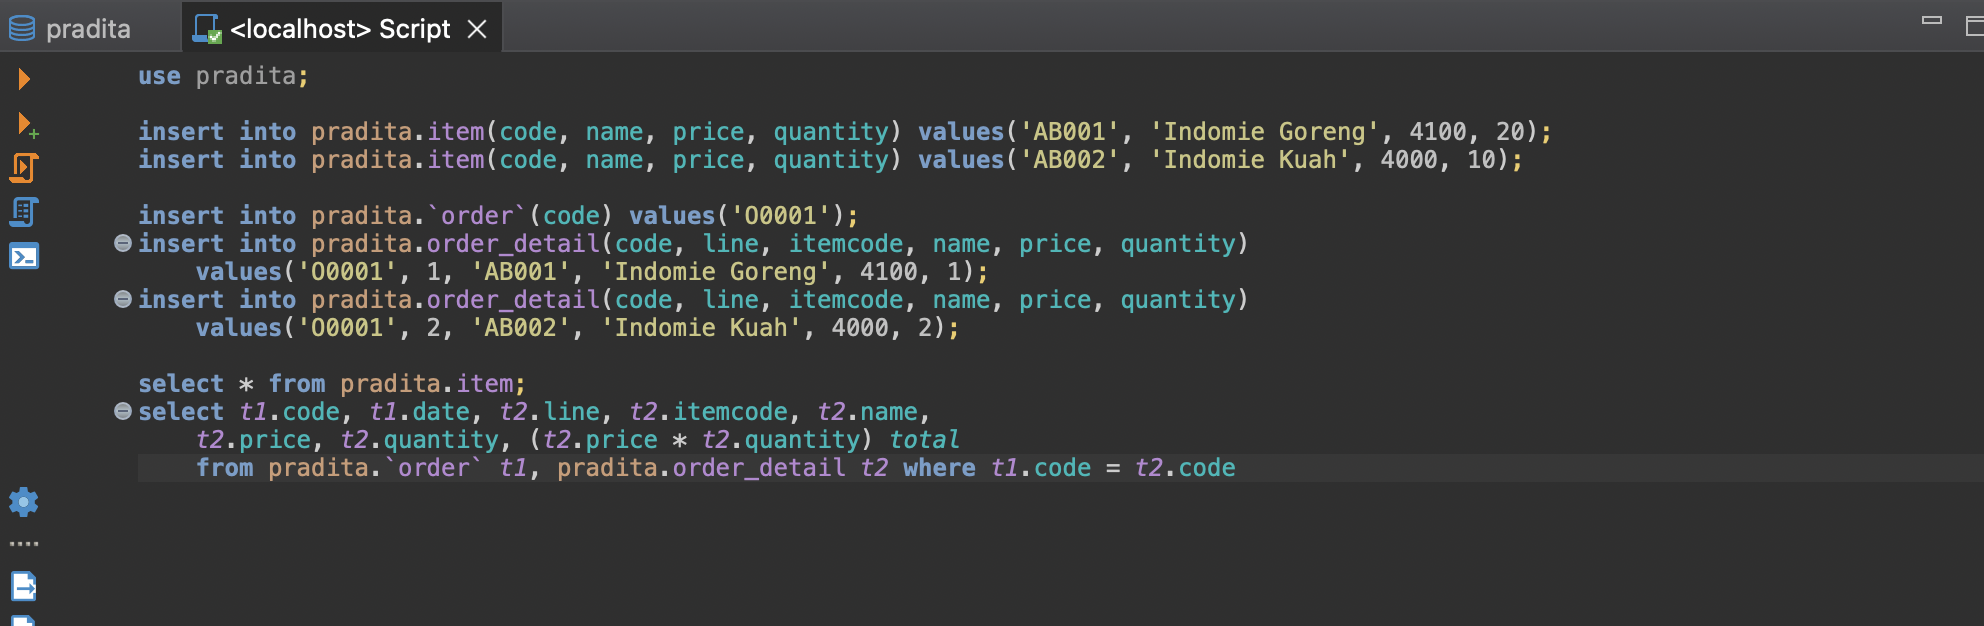
\includegraphics[width=1\textwidth]{assets/pertemuan12/dbeaver-database.png} 
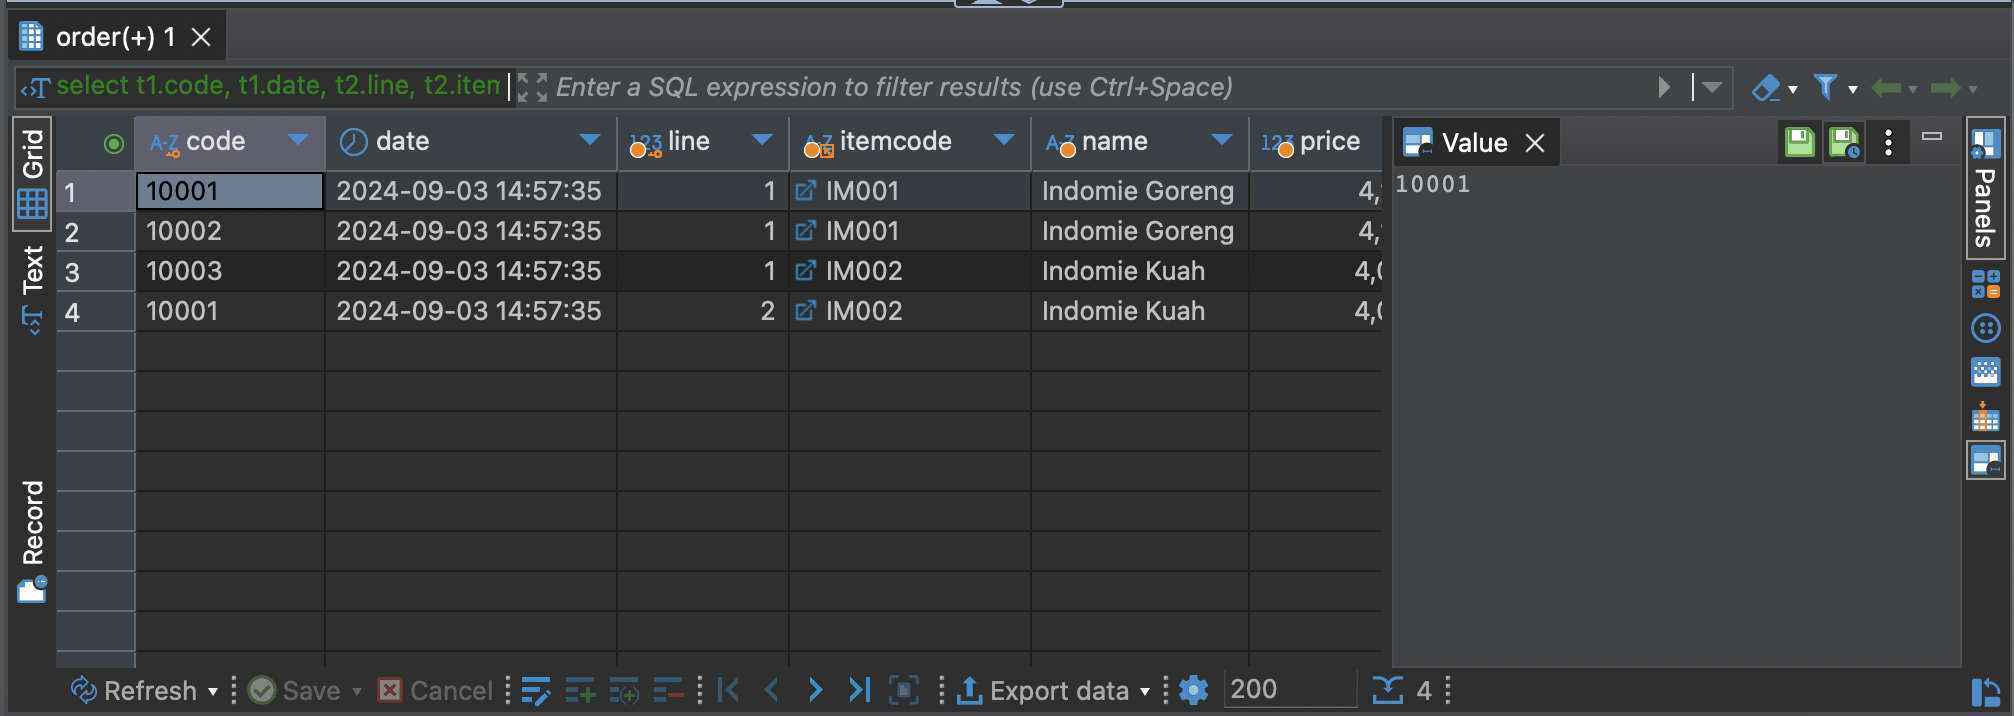
\includegraphics[width=1\textwidth]{assets/pertemuan12/dbeaver-success-script.png}

\subsubsection{Penjelasan Kode SQL}

Kode SQL yang diberikan bertujuan untuk membuat sebuah basis data bernama \texttt{pradita} dan beberapa tabel di dalamnya. 

\begin{itemize}
	\item \textbf{Membuat Basis Data:} Kode ini memastikan bahwa basis data \texttt{pradita} dibuat jika belum ada, kemudian menggunakannya.
	\item \textbf{Membuat Tabel \texttt{item}:} Tabel ini menyimpan informasi tentang barang dengan atribut \texttt{code} sebagai kunci utama, \texttt{name} untuk nama barang, \texttt{price} untuk harga barang, dan \texttt{quantity} untuk jumlah barang.
	\item \textbf{Membuat Tabel \texttt{order}:} Tabel ini menyimpan informasi pesanan dengan \texttt{code} sebagai kunci utama dan \texttt{date} yang merekam waktu pesanan dibuat.
	\item \textbf{Membuat Tabel \texttt{order\_detail}:} Tabel ini menghubungkan tabel \texttt{item} dan \texttt{order}, dengan atribut \texttt{code}, \texttt{line}, \texttt{itemcode}, \texttt{name}, \texttt{price}, dan \texttt{quantity}. Tabel ini juga menerapkan hubungan kunci asing (\textit{foreign key}) dengan tabel \texttt{item} dan \texttt{order}.
	\item \textbf{Memasukkan Data:} Kode juga memasukkan beberapa data ke dalam tabel \texttt{item}, \texttt{order}, dan \texttt{order\_detail}.
\end{itemize}

\subsection{Kode Java}

\subsubsection{Kelas TestConnection}

\begin{lstlisting}[style=JavaStyle]
	package edu.pradita.p12;
	
	import java.sql.Connection;
	import java.sql.DriverManager;
	import java.sql.ResultSet;
	import java.sql.SQLException;
	import java.sql.Statement;
	
	public class TestConnection {
		public static void main(String[] args) {
			try {
				Class.forName("com.mysql.cj.jdbc.Driver");
				Connection connection = DriverManager.getConnection("jdbc:mysql://localhost:3306/pradita", "root", "");
				
				Statement statement = connection.createStatement();
				ResultSet resultSet = statement.executeQuery("select * from item");
				while (resultSet.next()) {
					String code = resultSet.getString("code");
					String name = resultSet.getString("name");
					double price = resultSet.getDouble("price");
					double quantity = resultSet.getDouble("quantity");
					System.out.println(code + " " + name + " " + price + " " + ((int) quantity));
				}
				resultSet.close();
				statement.close();
				connection.close();
			} catch (ClassNotFoundException | SQLException e) {
				e.printStackTrace();
			}
		}
	}
\end{lstlisting}

\paragraph{1. Deklarasi Paket dan Import Library}
Kode dimulai dengan mendeklarasikan paket \texttt{edu.pradita.p12} dan mengimpor beberapa pustaka SQL dari Java seperti \texttt{Connection}, \texttt{DriverManager}, \texttt{ResultSet}, \texttt{SQLException}, dan \texttt{Statement}. Pustaka-pustaka ini digunakan untuk membuat koneksi ke basis data, menjalankan query SQL, dan menangani hasilnya.

\paragraph{2. Kelas \texttt{TestConnection}}
Kelas ini mendefinisikan \texttt{main} method, yang berfungsi sebagai titik masuk program. Tujuan utama dari kelas ini adalah melakukan koneksi ke basis data MySQL dan menampilkan data dari tabel tertentu.

\paragraph{3. Langkah-langkah dalam Kelas \texttt{TestConnection}}
\begin{itemize}
	\item \textbf{Memuat Driver JDBC}: Program pertama kali memuat driver JDBC untuk MySQL dengan menggunakan \texttt{Class.forName("com.mysql.cj.jdbc.Driver")}. Langkah ini diperlukan agar aplikasi dapat berkomunikasi dengan basis data MySQL.
	
	\item \textbf{Membuat Koneksi}: Menggunakan \texttt{DriverManager.getConnection} untuk membuat koneksi ke basis data \texttt{pradita} yang di-host di \texttt{localhost} pada port \texttt{3306}. Kredensial pengguna basis data, yaitu \texttt{"root"} tanpa kata sandi, disertakan dalam koneksi ini.
	
	\item \textbf{Membuat \texttt{Statement} dan Menjalankan Query}: 
	Objek \texttt{Statement} dibuat dari \texttt{Connection} untuk menjalankan pernyataan SQL. Query \texttt{SELECT * FROM item} dieksekusi untuk mengambil semua data dari tabel \texttt{item}.
	
	\item \textbf{Mengambil dan Menampilkan Data}: 
	Hasil dari query disimpan dalam \texttt{ResultSet} dan diproses dalam sebuah loop \texttt{while}. Pada setiap iterasi, data dari kolom \texttt{code}, \texttt{name}, \texttt{price}, dan \texttt{quantity} diambil dari \texttt{ResultSet} menggunakan metode seperti \texttt{getString} dan \texttt{getDouble}. Data ini kemudian ditampilkan ke konsol dengan \texttt{System.out.println}.
	
	\item \textbf{Menutup Koneksi dan Statement}: Setelah data selesai ditampilkan, \texttt{ResultSet}, \texttt{Statement}, dan \texttt{Connection} ditutup untuk membebaskan sumber daya.
\end{itemize}

\paragraph{4. Penanganan Exception}
Kode ini menangkap dua jenis \textit{exception} dengan menggunakan blok \texttt{try-catch}: 
\begin{itemize}
	\item \texttt{ClassNotFoundException} ditangani ketika driver JDBC MySQL tidak ditemukan.
	\item \texttt{SQLException} ditangani untuk menangkap kesalahan yang terjadi saat berinteraksi dengan basis data.
\end{itemize}

Jika salah satu \textit{exception} terjadi, program akan mencetak stack trace kesalahan tersebut ke konsol menggunakan \texttt{e.printStackTrace()}.

\paragraph{Kesimpulan}
Kode ini menunjukkan cara mendasar untuk menghubungkan aplikasi Java dengan basis data MySQL, mengeksekusi query SQL, dan menampilkan hasilnya. Struktur ini dapat digunakan untuk berbagai operasi dasar basis data seperti \textit{CRUD} (Create, Read, Update, Delete) pada aplikasi Java berbasis database.

\subsubsection{Kelas Order Form}

\begin{lstlisting}[style=JavaStyle]
	package edu.pradita.p12;
	
	import java.awt.EventQueue;
	
	import javax.swing.JFrame;
	import javax.swing.JScrollPane;
	import javax.swing.JTable;
	import javax.swing.table.DefaultTableModel;
	import javax.swing.JButton;
	import java.awt.Font;
	import javax.swing.JLabel;
	import javax.swing.JTextField;
	import javax.swing.JTextArea;
	import javax.swing.JPanel;
	import java.awt.BorderLayout;
	import java.awt.FlowLayout;
	import javax.swing.BoxLayout;
	import java.awt.Component;
	import java.awt.GridLayout;
	import javax.swing.SwingConstants;
	import java.awt.GridBagLayout;
	import java.awt.GridBagConstraints;
	import java.awt.Insets;
	import javax.swing.Box;
	import java.awt.Dimension;
	import javax.swing.ListSelectionModel;
	
	public class OrderForm {
		
		private JFrame frmOrderForm;
		private JTable table;
		private JTextField txtTotal;
		private JTextField txtCode;
		private JTextField txtDate;
		
		/**
		* Launch the application.
		*/
		public static void main(String[] args) {
			EventQueue.invokeLater(new Runnable() {
				public void run() {
					try {
						OrderForm window = new OrderForm();
						window.frmOrderForm.setVisible(true);
					} catch (Exception e) {
						e.printStackTrace();
					}
				}
			});
		}
		
		/**
		* Create the application.
		*/
		public OrderForm() {
			initialize();
		}
		
		/**
		* Initialize the contents of the frame.
		*/
		private void initialize() {
			frmOrderForm = new JFrame();
			frmOrderForm.setTitle("Order Form");
			frmOrderForm.setFont(new Font("Tahoma", Font.PLAIN, 16));
			frmOrderForm.getContentPane().setFont(new Font("Tahoma", Font.PLAIN, 16));
			frmOrderForm.setBounds(100, 100, 723, 421);
			frmOrderForm.setDefaultCloseOperation(JFrame.EXIT_ON_CLOSE);
			frmOrderForm.getContentPane().setLayout(new BorderLayout(0, 0));
			
			JScrollPane scrollPane = new JScrollPane();
			frmOrderForm.getContentPane().add(scrollPane, BorderLayout.CENTER);
			
			table = new JTable();
			table.setSelectionMode(ListSelectionModel.SINGLE_SELECTION);
			table.setFont(new Font("Tahoma", Font.PLAIN, 16));
			scrollPane.setViewportView(table);
			table.setModel(new DefaultTableModel(
			new Object[][] {
				{null, null, null, null, null, null},
			},
			new String[] {
				"No.", "Item Code", "Name", "Price", "Quantity", "Total"
			}
			) {
				/**
				* 
				*/
				private static final long serialVersionUID = 1L;
				Class[] columnTypes = new Class[] {
					Integer.class, String.class, String.class, Double.class, Double.class, Double.class
				};
				public Class getColumnClass(int columnIndex) {
					return columnTypes[columnIndex];
				}
			});
			
			JPanel southPanel = new JPanel();
			frmOrderForm.getContentPane().add(southPanel, BorderLayout.SOUTH);
			southPanel.setLayout(new GridLayout(0, 2, 0, 0));
			
			JPanel panel = new JPanel();
			FlowLayout flowLayout = (FlowLayout) panel.getLayout();
			flowLayout.setAlignment(FlowLayout.LEFT);
			panel.setAlignmentY(Component.TOP_ALIGNMENT);
			panel.setAlignmentX(Component.LEFT_ALIGNMENT);
			southPanel.add(panel);
			
			JLabel lblTotal = new JLabel("Total");
			lblTotal.setFont(new Font("Dialog", Font.BOLD, 20));
			panel.add(lblTotal);
			
			txtTotal = new JTextField();
			txtTotal.setFont(new Font("Dialog", Font.BOLD, 20));
			txtTotal.setEditable(false);
			txtTotal.setColumns(10);
			panel.add(txtTotal);
			
			JPanel panel_1 = new JPanel();
			FlowLayout flowLayout_1 = (FlowLayout) panel_1.getLayout();
			flowLayout_1.setAlignment(FlowLayout.RIGHT);
			southPanel.add(panel_1);
			
			JButton btnConfirm = new JButton("Confirm");
			btnConfirm.setFont(new Font("Tahoma", Font.PLAIN, 20));
			panel_1.add(btnConfirm);
			
			JPanel northPanel = new JPanel();
			frmOrderForm.getContentPane().add(northPanel, BorderLayout.NORTH);
			GridBagLayout gbl_northPanel = new GridBagLayout();
			gbl_northPanel.columnWidths = new int[]{709, 0};
			gbl_northPanel.rowHeights = new int[] {50, 78, 0};
			gbl_northPanel.columnWeights = new double[]{0.0, Double.MIN_VALUE};
			gbl_northPanel.rowWeights = new double[]{0.0, 0.0, Double.MIN_VALUE};
			northPanel.setLayout(gbl_northPanel);
			
			JPanel panel_2 = new JPanel();
			FlowLayout flowLayout_4 = (FlowLayout) panel_2.getLayout();
			flowLayout_4.setAlignment(FlowLayout.LEFT);
			GridBagConstraints gbc_panel_2 = new GridBagConstraints();
			gbc_panel_2.fill = GridBagConstraints.BOTH;
			gbc_panel_2.insets = new Insets(0, 0, 5, 0);
			gbc_panel_2.gridx = 0;
			gbc_panel_2.gridy = 0;
			northPanel.add(panel_2, gbc_panel_2);
			
			JButton btnNew = new JButton("New");
			btnNew.setFont(new Font("Tahoma", Font.PLAIN, 16));
			panel_2.add(btnNew);
			
			JButton btnFind = new JButton("Find");
			btnFind.setFont(new Font("Tahoma", Font.PLAIN, 16));
			panel_2.add(btnFind);
			
			JLabel lblNewLabel = new JLabel("Code");
			lblNewLabel.setFont(new Font("Tahoma", Font.PLAIN, 16));
			panel_2.add(lblNewLabel);
			
			txtCode = new JTextField();
			txtCode.setEditable(false);
			txtCode.setFont(new Font("Tahoma", Font.PLAIN, 16));
			txtCode.setColumns(10);
			panel_2.add(txtCode);
			
			Component rigidArea = Box.createRigidArea(new Dimension(100, 20));
			panel_2.add(rigidArea);
			
			JLabel lblDate = new JLabel("Date");
			lblDate.setFont(new Font("Tahoma", Font.PLAIN, 16));
			panel_2.add(lblDate);
			
			txtDate = new JTextField();
			txtDate.setEditable(false);
			txtDate.setFont(new Font("Tahoma", Font.PLAIN, 16));
			txtDate.setColumns(10);
			panel_2.add(txtDate);
			
			JPanel panel_4 = new JPanel();
			FlowLayout flowLayout_3 = (FlowLayout) panel_4.getLayout();
			flowLayout_3.setAlignment(FlowLayout.LEADING);
			GridBagConstraints gbc_panel_4 = new GridBagConstraints();
			gbc_panel_4.anchor = GridBagConstraints.SOUTH;
			gbc_panel_4.fill = GridBagConstraints.BOTH;
			gbc_panel_4.gridx = 0;
			gbc_panel_4.gridy = 1;
			northPanel.add(panel_4, gbc_panel_4);
			
			JButton btnAddItem = new JButton("Add Item");
			btnAddItem.setFont(new Font("Tahoma", Font.PLAIN, 16));
			panel_4.add(btnAddItem);
			
			JButton btnDeleteItem = new JButton("Remove Item");
			btnDeleteItem.setFont(new Font("Tahoma", Font.PLAIN, 16));
			panel_4.add(btnDeleteItem);
			
			Component rigidArea_1 = Box.createRigidArea(new Dimension(100, 20));
			panel_4.add(rigidArea_1);
			
			JLabel lblNote = new JLabel("Note");
			lblNote.setVerticalAlignment(SwingConstants.TOP);
			lblNote.setFont(new Font("Tahoma", Font.PLAIN, 16));
			panel_4.add(lblNote);
			
			JTextArea txtNote = new JTextArea();
			txtNote.setRows(3);
			txtNote.setColumns(30);
			panel_4.add(txtNote);
			table.getColumnModel().getColumn(0).setPreferredWidth(27);
			table.getColumnModel().getColumn(1).setPreferredWidth(64);
			table.getColumnModel().getColumn(2).setPreferredWidth(195);
			table.getColumnModel().getColumn(3).setPreferredWidth(68);
			table.getColumnModel().getColumn(4).setPreferredWidth(50);
			table.getColumnModel().getColumn(5).setPreferredWidth(108);
		}
	}
	
\end{lstlisting}

\paragraph{1. Package dan Import}
\begin{itemize}
	\item Baris pertama mendeklarasikan package \texttt{edu.pradita.p12}.
	\item Kode berikutnya mengimpor pustaka Java untuk antarmuka pengguna (\texttt{javax.swing.*}) dan elemen layout (\texttt{java.awt.*}) yang dibutuhkan.
\end{itemize}

\paragraph{2. Deklarasi Kelas \texttt{OrderForm}}
\begin{itemize}
	\item Kelas \texttt{OrderForm} merupakan kelas utama yang memiliki elemen-elemen antarmuka pengguna seperti \texttt{JFrame}, \texttt{JTable}, dan \texttt{JTextField}.
	\item Atribut yang digunakan antara lain:
	\begin{itemize}
		\item \texttt{frmOrderForm}: Objek \texttt{JFrame} utama yang menjadi wadah komponen antarmuka.
		\item \texttt{table}: Komponen tabel untuk menampilkan data pesanan.
		\item \texttt{txtTotal}, \texttt{txtCode}, \texttt{txtDate}: \texttt{JTextField} untuk menampilkan total harga, kode item, dan tanggal.
	\end{itemize}
\end{itemize}

\paragraph{3. \texttt{main} Method}
\begin{itemize}
	\item Method \texttt{main} menjalankan aplikasi dengan memanggil \texttt{OrderForm} dan menampilkannya menggunakan \texttt{EventQueue}.
\end{itemize}

\paragraph{4. Konstruktor \texttt{OrderForm}}
\begin{itemize}
	\item Konstruktor \texttt{OrderForm} memanggil method \texttt{initialize()} untuk mengatur antarmuka pengguna.
\end{itemize}

\paragraph{5. Method \texttt{initialize}}
\begin{itemize}
	\item Method ini berfungsi untuk mengatur komponen GUI.
	\item Berikut adalah komponen-komponen utama yang diatur dalam \texttt{initialize()}:
	
	\subparagraph{5.1. \texttt{JFrame} dan \texttt{JScrollPane}}
	\begin{itemize}
		\item \texttt{frmOrderForm} adalah objek \texttt{JFrame} utama. Di dalamnya terdapat \texttt{JScrollPane} yang menampung tabel untuk menampilkan data pesanan.
	\end{itemize}
	
	\subparagraph{5.2. \texttt{JTable} (Tabel)}
	\begin{itemize}
		\item \texttt{table}: Tabel menampilkan data pesanan dengan kolom seperti "No.", "Item Code", "Name", "Price", "Quantity", dan "Total".
		\item Model tabel diset menggunakan \texttt{DefaultTableModel} dengan tipe data yang didefinisikan pada masing-masing kolom.
	\end{itemize}
	
	\subparagraph{5.3. Panel Bagian Bawah (South Panel)}
	\begin{itemize}
		\item Terdapat dua panel dalam bagian bawah untuk menampilkan \texttt{Total} dan \texttt{Confirm} button.
		\item Label \texttt{Total} dan field \texttt{txtTotal} untuk menampilkan total harga pesanan.
	\end{itemize}
	
	\subparagraph{5.4. Panel Bagian Atas (North Panel)}
	\begin{itemize}
		\item Panel ini berisi tombol-tombol \texttt{New}, \texttt{Find}, \texttt{Add Item}, dan \texttt{Remove Item}.
		\item Selain itu, terdapat input \texttt{txtCode}, \texttt{txtDate}, dan area teks \texttt{txtNote} untuk menambahkan catatan.
	\end{itemize}
\end{itemize}

\paragraph{Kesimpulan}
Kode ini membentuk antarmuka untuk formulir pemesanan dengan fitur tabel data, kalkulasi total harga, dan area catatan. Struktur layout yang digunakan memungkinkan pengaturan posisi komponen yang fleksibel dengan bantuan \texttt{BorderLayout}, \texttt{GridLayout}, dan \texttt{FlowLayout}.


\subsubsection{Kelas Select Form}

\begin{lstlisting}[style=JavaStyle]
	package edu.pradita.p12;
	
	import java.awt.BorderLayout;
	import java.awt.EventQueue;
	
	import javax.swing.JFrame;
	import javax.swing.JPanel;
	import javax.swing.border.EmptyBorder;
	import java.awt.Font;
	import javax.swing.JLabel;
	import javax.swing.JTextField;
	import javax.swing.JTable;
	import javax.swing.JScrollPane;
	import javax.swing.table.DefaultTableModel;
	import javax.swing.JButton;
	import javax.swing.BoxLayout;
	import java.awt.Component;
	import java.awt.GridLayout;
	import javax.swing.SwingConstants;
	import java.awt.GridBagLayout;
	import java.awt.GridBagConstraints;
	import java.awt.Insets;
	import javax.swing.ListSelectionModel;
	
	public class SelectForm extends JFrame {
		
		private JPanel contentPane;
		private JTable table;
		private JTextField textField;
		
		/**
		* Launch the application.
		*/
		public static void main(String[] args) {
			EventQueue.invokeLater(new Runnable() {
				public void run() {
					try {
						SelectForm frame = new SelectForm();
						frame.setVisible(true);
					} catch (Exception e) {
						e.printStackTrace();
					}
				}
			});
		}
		
		/**
		* Create the frame.
		*/
		public SelectForm() {
			setTitle("Select Form");
			setFont(new Font("Tahoma", Font.PLAIN, 16));
			setDefaultCloseOperation(JFrame.EXIT_ON_CLOSE);
			setBounds(100, 100, 350, 270);
			contentPane = new JPanel();
			contentPane.setBorder(new EmptyBorder(5, 5, 5, 5));
			setContentPane(contentPane);
			contentPane.setLayout(new BorderLayout(0, 4));
			
			JPanel panel = new JPanel();
			contentPane.add(panel, BorderLayout.SOUTH);
			panel.setLayout(new GridLayout(1, 2, 0, 0));
			
			JButton btnCancel = new JButton("Cancel");
			btnCancel.setAlignmentX(Component.CENTER_ALIGNMENT);
			btnCancel.setAlignmentY(Component.BOTTOM_ALIGNMENT);
			btnCancel.setFont(new Font("Tahoma", Font.PLAIN, 16));
			panel.add(btnCancel);
			
			JButton btnNewButton = new JButton("OK");
			btnNewButton.setAlignmentX(Component.CENTER_ALIGNMENT);
			btnNewButton.setFont(new Font("Tahoma", Font.PLAIN, 16));
			panel.add(btnNewButton);
			
			JScrollPane scrollPane = new JScrollPane();
			contentPane.add(scrollPane, BorderLayout.CENTER);
			
			table = new JTable();
			table.setFont(new Font("Tahoma", Font.PLAIN, 16));
			table.setSelectionMode(ListSelectionModel.SINGLE_SELECTION);
			table.setEnabled(false);
			table.setModel(new DefaultTableModel(
			new Object[][] {
				{null, null},
			},
			new String[] {
				"Code", "Description"
			}
			) {
				Class[] columnTypes = new Class[] {
					String.class, String.class
				};
				public Class getColumnClass(int columnIndex) {
					return columnTypes[columnIndex];
				}
			});
			table.getColumnModel().getColumn(0).setPreferredWidth(71);
			table.getColumnModel().getColumn(1).setPreferredWidth(204);
			scrollPane.setViewportView(table);
			
			JPanel panel_1 = new JPanel();
			contentPane.add(panel_1, BorderLayout.NORTH);
			panel_1.setLayout(new BorderLayout(10, 0));
			
			JLabel lblFind = new JLabel("Find:");
			lblFind.setFont(new Font("Tahoma", Font.PLAIN, 16));
			panel_1.add(lblFind, BorderLayout.WEST);
			
			textField = new JTextField();
			lblFind.setLabelFor(textField);
			textField.setFont(new Font("Tahoma", Font.PLAIN, 16));
			textField.setColumns(10);
			panel_1.add(textField);
			
			JButton btnFind = new JButton("Find");
			btnFind.setFont(new Font("Tahoma", Font.PLAIN, 16));
			panel_1.add(btnFind, BorderLayout.EAST);
		}
		
	}
\end{lstlisting}


\paragraph{1. Deklarasi Paket dan Import Library}
Kode ini dimulai dengan mendeklarasikan paket \texttt{edu.pradita.p12} dan mengimpor beberapa pustaka dari \textit{Swing} dan \textit{AWT} untuk membuat antarmuka grafis. Beberapa pustaka utama yang digunakan adalah \texttt{JFrame}, \texttt{JTable}, dan \texttt{JScrollPane}.

\paragraph{2. Kelas \texttt{SelectForm}}
Kelas \texttt{SelectForm} diperluas dari \texttt{JFrame}, yang memungkinkan untuk membuat jendela utama aplikasi GUI. Berikut komponen-komponen utama di dalamnya:

\begin{itemize}
	\item \texttt{JPanel} dan \texttt{contentPane}: Panel utama dengan tata letak \texttt{BorderLayout} yang berfungsi sebagai kontainer untuk komponen lain di jendela.
	\item \texttt{JTable}: Komponen untuk menampilkan data dalam bentuk tabel. Tabel ini diatur agar tidak dapat diedit (\texttt{setEnabled(false)}) dan menggunakan \texttt{DefaultTableModel} dengan dua kolom: \textit{Code} dan \textit{Description}.
\end{itemize}

\paragraph{3. Metode \texttt{main}}
Metode ini berfungsi sebagai titik masuk aplikasi. \texttt{EventQueue.invokeLater} digunakan untuk menjalankan aplikasi dalam \textit{event-dispatching thread}, yang diperlukan untuk aplikasi GUI berbasis \texttt{Swing}.

\paragraph{4. Konstruktor \texttt{SelectForm}}
Konstruktor ini menginisialisasi komponen GUI dalam jendela utama:
\begin{itemize}
	\item \textbf{Tata Letak Utama dan Ukuran Jendela}: Menyetel judul jendela, font, operasi \texttt{EXIT\_ON\_CLOSE}, dan ukuran jendela.
	\item \textbf{Panel Selatan (\texttt{panel})}: Digunakan untuk menempatkan dua tombol, yaitu \texttt{OK} dan \texttt{Cancel}, dengan \texttt{GridLayout} 1x2 untuk menata tombol secara horizontal.
	\item \textbf{\texttt{JTable} dalam \texttt{JScrollPane}}: \texttt{JScrollPane} digunakan untuk memungkinkan tabel di-\texttt{scroll} bila datanya lebih banyak dari ukuran jendela. Tabel ini menampilkan dua kolom dengan data kosong.
	\item \textbf{Panel Pencarian}: Bagian atas jendela memiliki label "Find", kolom input teks (\texttt{JTextField}), dan tombol "Find". Bagian ini memungkinkan pengguna untuk memasukkan kata kunci pencarian untuk mencari data di tabel.
\end{itemize}

\paragraph{5. Interaksi Pengguna}
Kode ini mendefinisikan elemen interaktif seperti tombol \texttt{OK}, \texttt{Cancel}, dan \texttt{Find}. Pada kode ini, fungsionalitas tombol tersebut belum diimplementasikan, sehingga hanya elemen antarmuka yang terlihat.

\paragraph{Kesimpulan}
Kode ini membangun antarmuka dasar untuk aplikasi pencarian dengan tabel menggunakan \texttt{Swing}. Meskipun belum memiliki logika pencarian yang sebenarnya, struktur dasar seperti tabel dan panel pencarian telah siap digunakan.


\section{Soal Studi Kasus}

\subsection{Pembuatan Database Sederhana untuk Sistem Perpustakaan}
Dalam studi kasus ini, kita akan membuat skema database sederhana untuk sistem perpustakaan menggunakan SQL. Database ini akan terdiri dari tiga tabel utama: \texttt{Buku}, \texttt{Anggota}, dan \texttt{Peminjaman}. Setiap tabel akan memiliki kolom khusus yang memungkinkan kita untuk mengelola informasi buku, anggota perpustakaan, dan riwayat peminjaman.

\begin{itemize}
	\item \textbf{Tabel Buku}:
	\begin{itemize}
		\item Tabel ini berfungsi untuk menyimpan informasi tentang buku yang tersedia di perpustakaan.
		\item Kolom yang dibutuhkan antara lain \texttt{ID\_Buku}, \texttt{Judul}, \texttt{Penulis}, dan \texttt{Tahun\_Terbit}.
	\end{itemize}
	
	\item \textbf{Tabel Anggota}:
	\begin{itemize}
		\item Tabel ini berfungsi untuk menyimpan informasi tentang anggota perpustakaan.
		\item Kolom yang dibutuhkan antara lain \texttt{ID\_Anggota}, \texttt{Nama}, \texttt{Alamat}, dan \texttt{Nomor\_Telepon}.
	\end{itemize}
	
	\item \textbf{Tabel Peminjaman}:
	\begin{itemize}
		\item Tabel ini mencatat transaksi peminjaman buku oleh anggota.
		\item Kolom yang dibutuhkan antara lain \texttt{ID\_Peminjaman}, \texttt{ID\_Buku}, \texttt{ID\_Anggota}, \texttt{Tanggal\_Pinjam}, dan \texttt{Tanggal\_Kembali}.
	\end{itemize}
\end{itemize}

\subsubsection{Instruksi Studi Kasus}
Tugas Anda adalah untuk menulis kode SQL yang:

\begin{enumerate}
	\item Membuat database dengan nama \texttt{Perpustakaan}.
	\item Membuat tabel \texttt{Buku}, \texttt{Anggota}, dan \texttt{Peminjaman} dengan kolom-kolom yang telah disebutkan.
	\item Menetapkan \texttt{primary key} pada masing-masing tabel.
	\item Menambahkan \texttt{foreign key} yang sesuai untuk menghubungkan tabel \texttt{Peminjaman} dengan tabel \texttt{Buku} dan \texttt{Anggota}.
	\item Memasukkan setidaknya tiga data contoh ke dalam masing-masing tabel.
	\item Setelah membuat database, gunakan bahasa pemrograman Java untuk melakukan tes koneksi pada database berikut.
\end{enumerate}

Pada akhir studi kasus ini, Anda akan memiliki database \texttt{Perpustakaan} yang dapat digunakan untuk mengelola informasi buku, anggota, dan transaksi peminjaman buku.
